\section{Linguaggi di interrogazione nei sistemi NoSql}
Nei sistemi NoSqlspesso non sono disponibili veri e propri linguaggi di interrogazione come nei sistemi relazionali.
Solo i sistemi document-based forniscono strumenti simili all'algebra e al calcolo relazionale per l'accesso ai dati.
\begin{figure}[H]
	\centering
	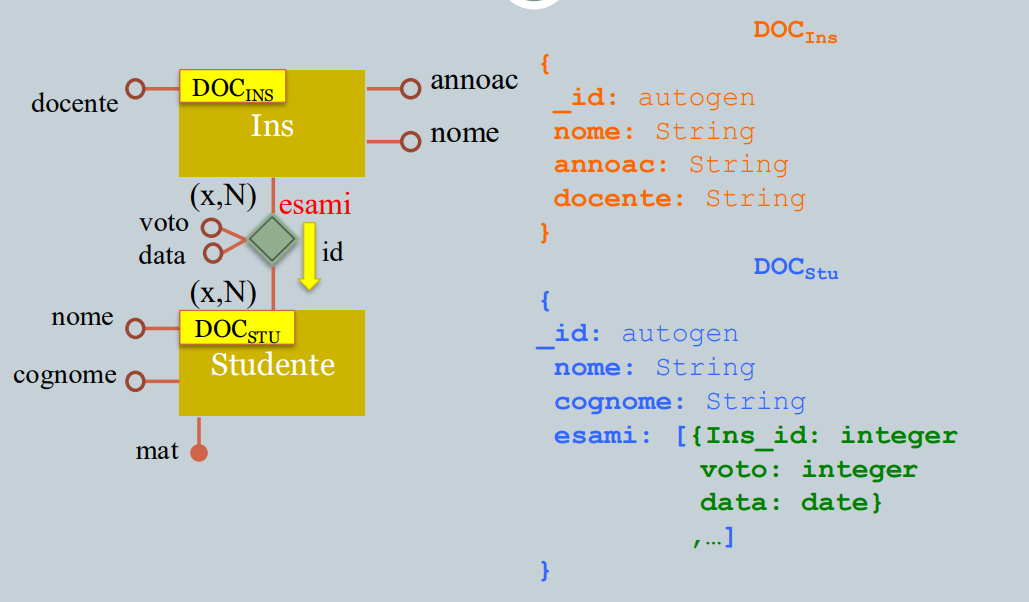
\includegraphics[width=1\linewidth]{image99}
	\caption{esempio sistemi document-store}
	\label{fig:image99}
\end{figure}
La maggior parte del linguaggio di interrogazione di MongoDB è realizzato attraverso il metodo find.
\begin{figure}[H]
	\centering
	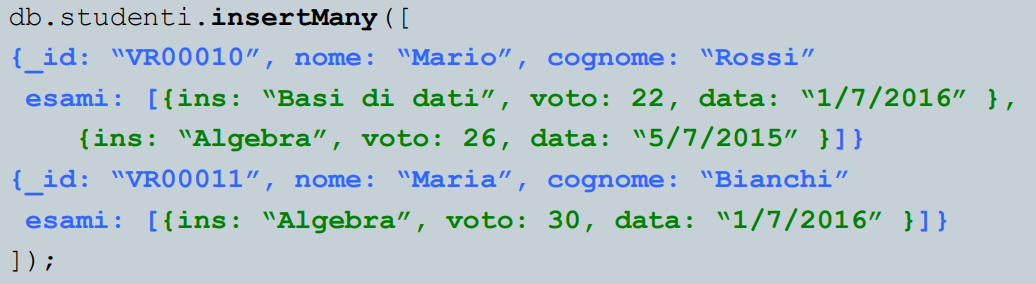
\includegraphics[width=1\linewidth]{image100}
	\caption{esempio con mongo db del document based di prima}
	\label{fig:image100}
\end{figure}
\begin{figure}[H]
	\centering
	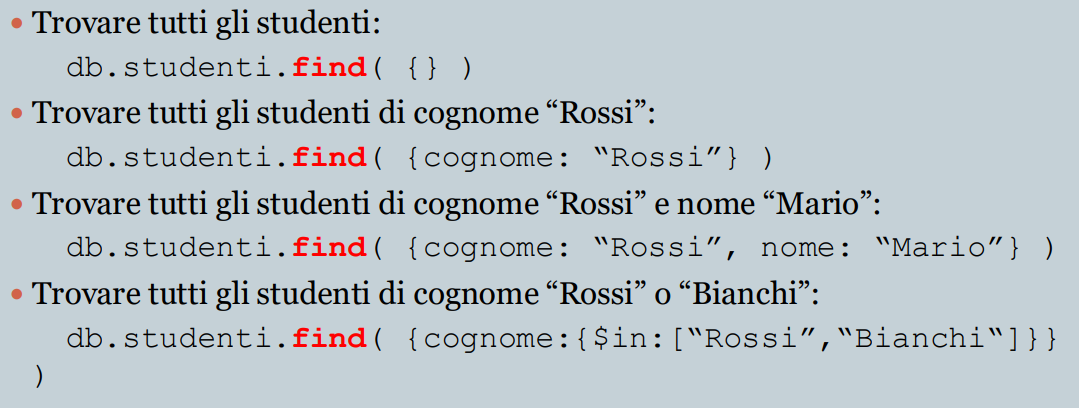
\includegraphics[width=1\linewidth]{image101}
	\caption{Interrogazioni Semplici}
	\label{fig:image101}
\end{figure}
\begin{figure}[H]
	\centering
	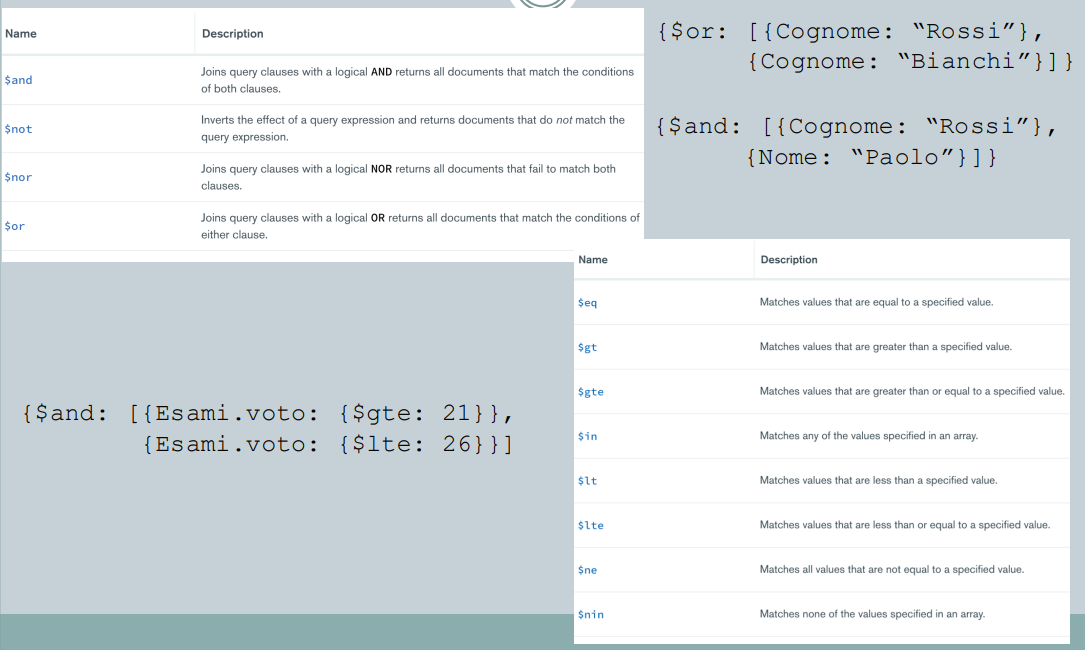
\includegraphics[width=1\linewidth]{image102}
	\caption{Operatori di Confronto}
	\label{fig:image102}
\end{figure}
\begin{figure}[H]
	\centering
	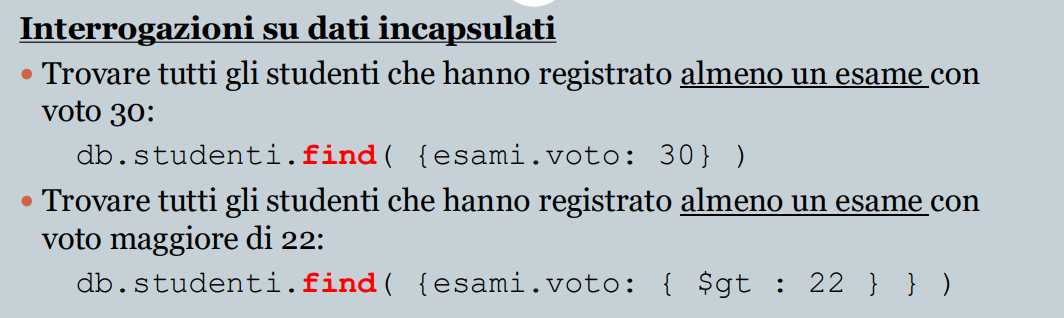
\includegraphics[width=1\linewidth]{image103}
	\caption{Esempio di interrogazioni con gli operatori}
	\label{fig:image103}
\end{figure}
\begin{figure}[H]
	\centering
	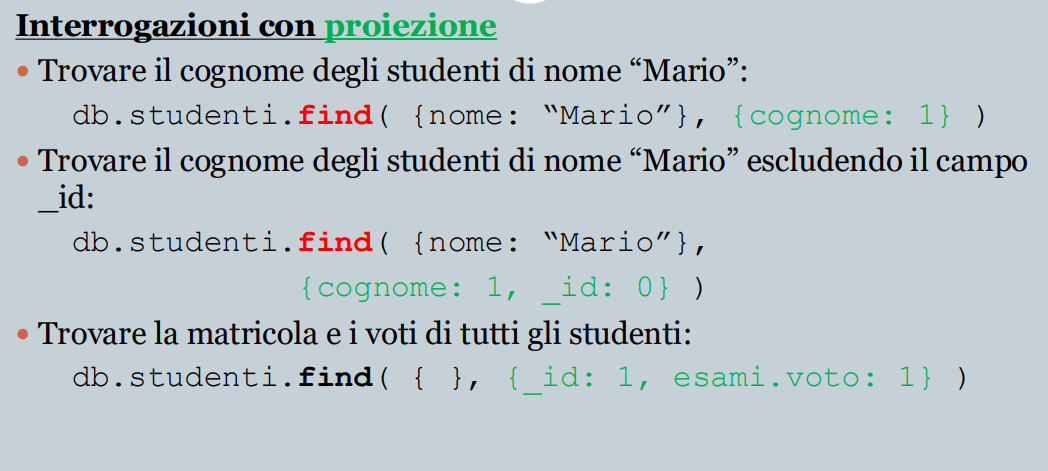
\includegraphics[width=1\linewidth]{image104}
	\caption{Interrogazioni con proiezione}
	\label{fig:image104}
\end{figure}
\begin{figure}[H]
	\centering
	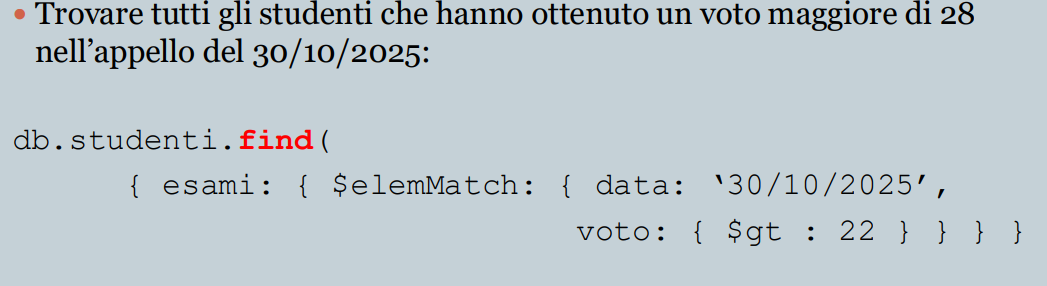
\includegraphics[width=1\linewidth]{image105}
	\caption{condizioni multiple}
	\label{fig:image105}
\end{figure}
